\documentclass[12pt,a4paper]{article}

% --- Packages ---
\usepackage[american]{babel}
\usepackage{amsmath,amssymb}
\usepackage{setspace}
\usepackage[margin=1in]{geometry}
\usepackage[T1]{fontenc}
\usepackage{times}
\usepackage[numbers,sort&compress]{natbib}
\usepackage{graphicx}
\usepackage[hyphens]{url}
\usepackage[hidelinks]{hyperref}
\usepackage{booktabs}
\usepackage{tabularx}
\usepackage{caption}
\usepackage{float}
\usepackage{enumitem}

% --- Formatting ---
\doublespacing
\setlength{\parindent}{0.5in}
\bibliographystyle{unsrtnat}

% --- Title Page ---
\title{\textbf{Cost-Effectiveness of Intismeran Autogene Plus Pembrolizumab Versus Pembrolizumab Alone as Adjuvant Therapy for Resected Stage IIIB–IV Melanoma: An Updated Early Economic Evaluation}}

\author{Yichao Jin, Ph.D. \\
  School of Economic, Political and Policy Sciences, \\
  University of Texas at Dallas, Richardson, TX, USA \\
  \texttt{Yichao.Jin@UTDallas.edu} \\
  ORCID: 0009-0003-7667-5143}

\date{}

\begin{document}
\tolerance=2000
\emergencystretch=3em
\hfuzz=1pt

\maketitle
\thispagestyle{empty}

{\noindent\small
\textbf{Funding:} This study was conducted without external funding.

\textbf{Acknowledgments:} None.

\textbf{Conflict of interest:} The author declares no competing interests relevant to this study.

\textbf{Reporting:} This study adheres to the Consolidated Health Economic Evaluation Reporting Standards 2022 (CHEERS 2022) \cite{husereau2022} (Supplementary Checklist).

\textbf{Data and code availability:} All data used in this analysis are derived from published sources cited in the references. The model code is available at \url{https://github.com/yichao2022/cea-intismeran}.
}

\newpage

% --- Abstract ---
\begingroup
\onehalfspacing
\emergencystretch=2em
\hyphenpenalty=10000
\exhyphenpenalty=10000
\setlength{\parindent}{0pt}
\begin{center}
{\large\bfseries Abstract}
\end{center}

\textbf{Background:} In August 2026, Merck and Moderna reported positive Phase 3 \mbox{INTerpath-001} results for intismeran autogene (mRNA-4157/V940) plus \mbox{pembrolizumab} in resected stage IIB--IV melanoma. Its cost-effectiveness remains unknown.

\textbf{Objective:} To estimate the cost-effectiveness of intismeran plus \mbox{pembrolizumab} versus \mbox{pembrolizumab} alone from a US payer perspective.

\textbf{Methods:} A four-state partitioned survival model was developed with a 40-year horizon and 3\% annual discounting. Quantitative efficacy inputs were derived from the Phase 2b \mbox{KEYNOTE-942} trial (n=157), with exploratory OS; Phase 3 \mbox{INTerpath-001} results were used as clinical context because numerical effect estimates were not yet available. Health-state utilities were drawn from published EQ-5D literature. Probabilistic, deterministic, and scenario sensitivity analyses were conducted.

\textbf{Results:} In the base case, intismeran plus \mbox{pembrolizumab} yielded 11.35 QALYs at a cost of \$874,026 versus 7.33 QALYs at \$712,110 for \mbox{pembrolizumab} alone. The ICER was \$40,274/QALY (incremental cost \$161,916). Probabilities of cost-effectiveness were 95.3\% at \$100,000 and 98.7\% at \$150,000/QALY. The deterministic threshold prices were approximately \$440K and \$641K. Results were largely robust across structural scenarios; the ICER exceeded \$100,000/QALY only under hazard-convergence waning (\$104,852/QALY).

\textbf{Conclusion:} At an estimated acquisition price of \$200,000 per course, intismeran plus \mbox{pembrolizumab} was projected to be cost-effective under conventional US thresholds, driven by a substantial but not implausibly large 4.02-QALY gain despite higher acquisition and treatment-related costs.

\noindent\parbox{0.94\linewidth}{\textbf{Keywords:} cost-effectiveness analysis, intismeran, mRNA-4157, V940, melanoma, \mbox{pembrolizumab}, Keytruda, individualized neoantigen therapy, partitioned survival model}

\endgroup

\newpage

% --- Body ---
\doublespacing

\section{Introduction}

\subsection{A New Reimbursement Problem}

On August 19, 2026, Merck and Moderna announced positive topline results from the Phase 3 \mbox{INTerpath-001} trial, establishing intismeran autogene (mRNA-4157/V940) plus \mbox{pembrolizumab} as the first mRNA-based individualized neoantigen therapy (INT) to succeed in a late-stage trial \cite{merck2026}. The press release confirmed statistically significant improvements in RFS and DMFS, though numerical hazard ratios have not yet been disclosed. This breakthrough follows the Phase 2b \mbox{KEYNOTE-942} trial, which at 5-year follow-up reported a sustained RFS benefit (HR 0.51, 95\% CI 0.294--0.887), DMFS benefit (HR 0.411, 95\% CI 0.200--0.843), and 5-year OS rates of 92.2\% (combo) versus 71.3\% (\mbox{pembrolizumab} alone; OS HR 0.471, 95\% CI 0.165--1.345) \cite{khattak2026}.

Despite these clinical advances, the economic implications of INTs remain poorly understood. These therapies combine the high costs of immune checkpoint inhibitors with the additional expense of individualized manufacturing, creating a reimbursement challenge unlike any in oncology.

\subsection{Why INTs Differ from Conventional Oncology Pricing}

Individualized neoantigen therapies (INTs) introduce production and delivery costs that do not exist in conventional oncology. Unlike fixed-composition drugs, each INT treatment is custom-manufactured for a single patient based on tumor sequencing data, requiring mRNA synthesis, lipid nanoparticle formulation, and quality assurance for each batch \cite{ibragimova2025, li2026}. These costs scale with each new patient rather than benefiting from traditional manufacturing economies of scale.

Jefferies analysts have estimated the cost of such vaccines at \$100,000--\$300,000 per patient \cite{jefferies2026}. By comparison, cancer immunotherapies such as Keytruda\textregistered{} (\mbox{pembrolizumab}) have annual costs of approximately \$220,896 in the adjuvant setting \cite{keytruda2026}. The combination of a high-cost immunotherapy with an individualized vaccine creates a compound affordability challenge for payers, particularly in the adjuvant setting where patients are recurrence-free at the time of treatment.

\subsection{Existing Economic Evidence}

A prior exploratory cost-effectiveness analysis of V940 plus \mbox{pembrolizumab} in adjuvant melanoma was presented at ISPOR 2024 \cite{mclean2024}. That analysis, conducted before the \mbox{KEYNOTE-942} 5-year results and the Phase 3 \mbox{INTerpath-001} readout, used a 4-state model with assumptions based on Phase 2b interim data. The analysis reported an ICER of approximately \$75,000/QALY, but relied on early efficacy estimates and assumed a V940 price equal to \mbox{pembrolizumab}, which may not reflect the likely INT premium. The present analysis updates these findings by incorporating the mature 5-year \mbox{KEYNOTE-942} data, applying a ratio-constrained partition survival structure with a general-population hazard floor, and conducting a comprehensive deterministic threshold price analysis.

\subsection{Clinical Basis and Research Objectives}

The clinical foundation for this analysis comes from the 5-year follow-up of the Phase 2b \mbox{KEYNOTE-942} trial, which provides the most mature efficacy data available for intismeran \cite{khattak2026}. The trial randomized 157 patients with completely resected stage IIIB--IV melanoma 2:1 to intismeran plus \mbox{pembrolizumab} or \mbox{pembrolizumab} alone. The primary endpoint was RFS; secondary endpoints included DMFS, OS, and safety. At the 5-year analysis, the combination showed a sustained RFS benefit with a hazard ratio of 0.51 (95\% CI 0.294--0.887), a DMFS HR of 0.411 (95\% CI 0.200--0.843), and OS data still maturing with 5-year OS rates of 92.2\% (combo) versus 71.3\% (\mbox{pembrolizumab} alone; OS HR 0.471, 95\% CI 0.165--1.345).

This study presents an early economic evaluation of intismeran plus \mbox{pembrolizumab} versus \mbox{pembrolizumab} alone as adjuvant therapy for completely resected stage IIIB--IV melanoma from a US payer perspective. Model efficacy inputs are derived from the Phase 2b \mbox{KEYNOTE-942} trial; Phase 3 \mbox{INTerpath-001} numerical data will be incorporated when available. We incorporate the latest \mbox{KEYNOTE-942} 5-year data, a calibrated parametric survival framework with internal consistency constraints, and a comprehensive range of sensitivity and scenario analyses to address the uncertainty inherent in early economic evaluations.

\section{Methods}

\subsection{Model Structure}

A partitioned survival model (PSM) was developed in Python with four mutually exclusive health states: recurrence-free (RF), locoregional recurrence (LR), distant metastasis (DM), and death, following the structure of prior melanoma cost-effectiveness models and standard PSM methodology \cite{woods2017,zhang2023,bensimon2019,gye2024}. Patients enter the model in the RF state and transition through LR and/or DM states based on parametric survival functions:
\begin{align*}
\text{RF}(t) &= \text{RFS}(t) \\
\text{LR}(t) &= \text{DMFS}(t) - \text{RFS}(t) \\
\text{DM}(t) &= \text{OS}(t) - \text{DMFS}(t) \\
\text{Dead}(t) &= 1 - \text{OS}(t)
\end{align*}
This construction ensures RFS $\leq$ DMFS $\leq$ OS at all times and maintains internal consistency without forcing a specific parametric form on the transition hazards.

\subsection{Clinical Data}

RFS and OS survival probabilities were extracted at 18, 24, 36, 48, and 60 months, and DMFS probabilities at 18, 24, 36, and 48 months, from the published \mbox{KEYNOTE-942} Kaplan--Meier curves \cite{khattak2026} (60-month DMFS was not reported in the 5-year analysis). Parametric survival models were fitted to these data points using weighted nonlinear least squares, following standard methodological guidance for survival extrapolation in health economic evaluation \cite{latimer2011,latimer2013,ishak2013}. Model selection was performed by comparing five candidate distributions (exponential, Weibull, log-normal, log-logistic, generalized gamma) for each of the three underlying survival components (OS, $r_{\text{DM}} = \text{DMFS}/\text{OS}$, $r_{\text{LR}} = \text{RFS}/\text{DMFS}$) using Akaike Information Criterion (AIC), as recommended by NICE DSU TSD 14 \cite{latimer2011}. All five candidate distributions (including the three-parameter generalized gamma) were evaluated across all six component--arm combinations (Supplementary Table~S3). A full joint enumeration of $5^6 = 15,625$ distribution combinations was performed (Supplementary Table~S4); the generalized gamma achieved the lowest component-level AIC for the r_{\text{DM}}--pembrolizumab component and appeared in all top-10 joint models. The log-normal distribution was selected as the base case because it achieved the best AIC for the OS curve of the combination arm (the most influential curve driving lifetime costs and QALYs) and was broadly competitive across other components. All 15,625 candidate combinations preserved the structural ordering constraint RFS $\leq$ DMFS $\leq$ OS at 40 years, so the choice of distribution was not driven by feasibility constraints. A common log-normal family was chosen for parsimony and interpretability; component-specific best-fitting distributions (Weibull, log-logistic) were examined in scenario analyses. The fitted model was calibrated to ensure the constraint RFS $\leq$ DMFS $\leq$ OS was satisfied at all time points. To address the external validity of long-term survival extrapolation, a general population mortality hazard floor was applied from 60 months onward, using the age- and sex-matched US 2019 life table (pooled 64\% male/36\% female, baseline age 61 years) \cite{arias2022}. This constraint ensures that the model does not produce survival probabilities exceeding those of the general population at any time point, a standard practice in oncology cost-effectiveness analyses \cite{latimer2011,zhang2023}.

\subsection{External Validation}
Model predictions for the \mbox{pembrolizumab}-alone arm were externally validated against the KEYNOTE-054 and CheckMate 238 trials (Section~3.3).
Figure~\ref{fig:survival} illustrates the fitted RFS, DMFS, and OS trajectories for both treatment arms together with the observed \mbox{KEYNOTE-942} landmark data used for calibration.

\begin{figure}[H]
\centering
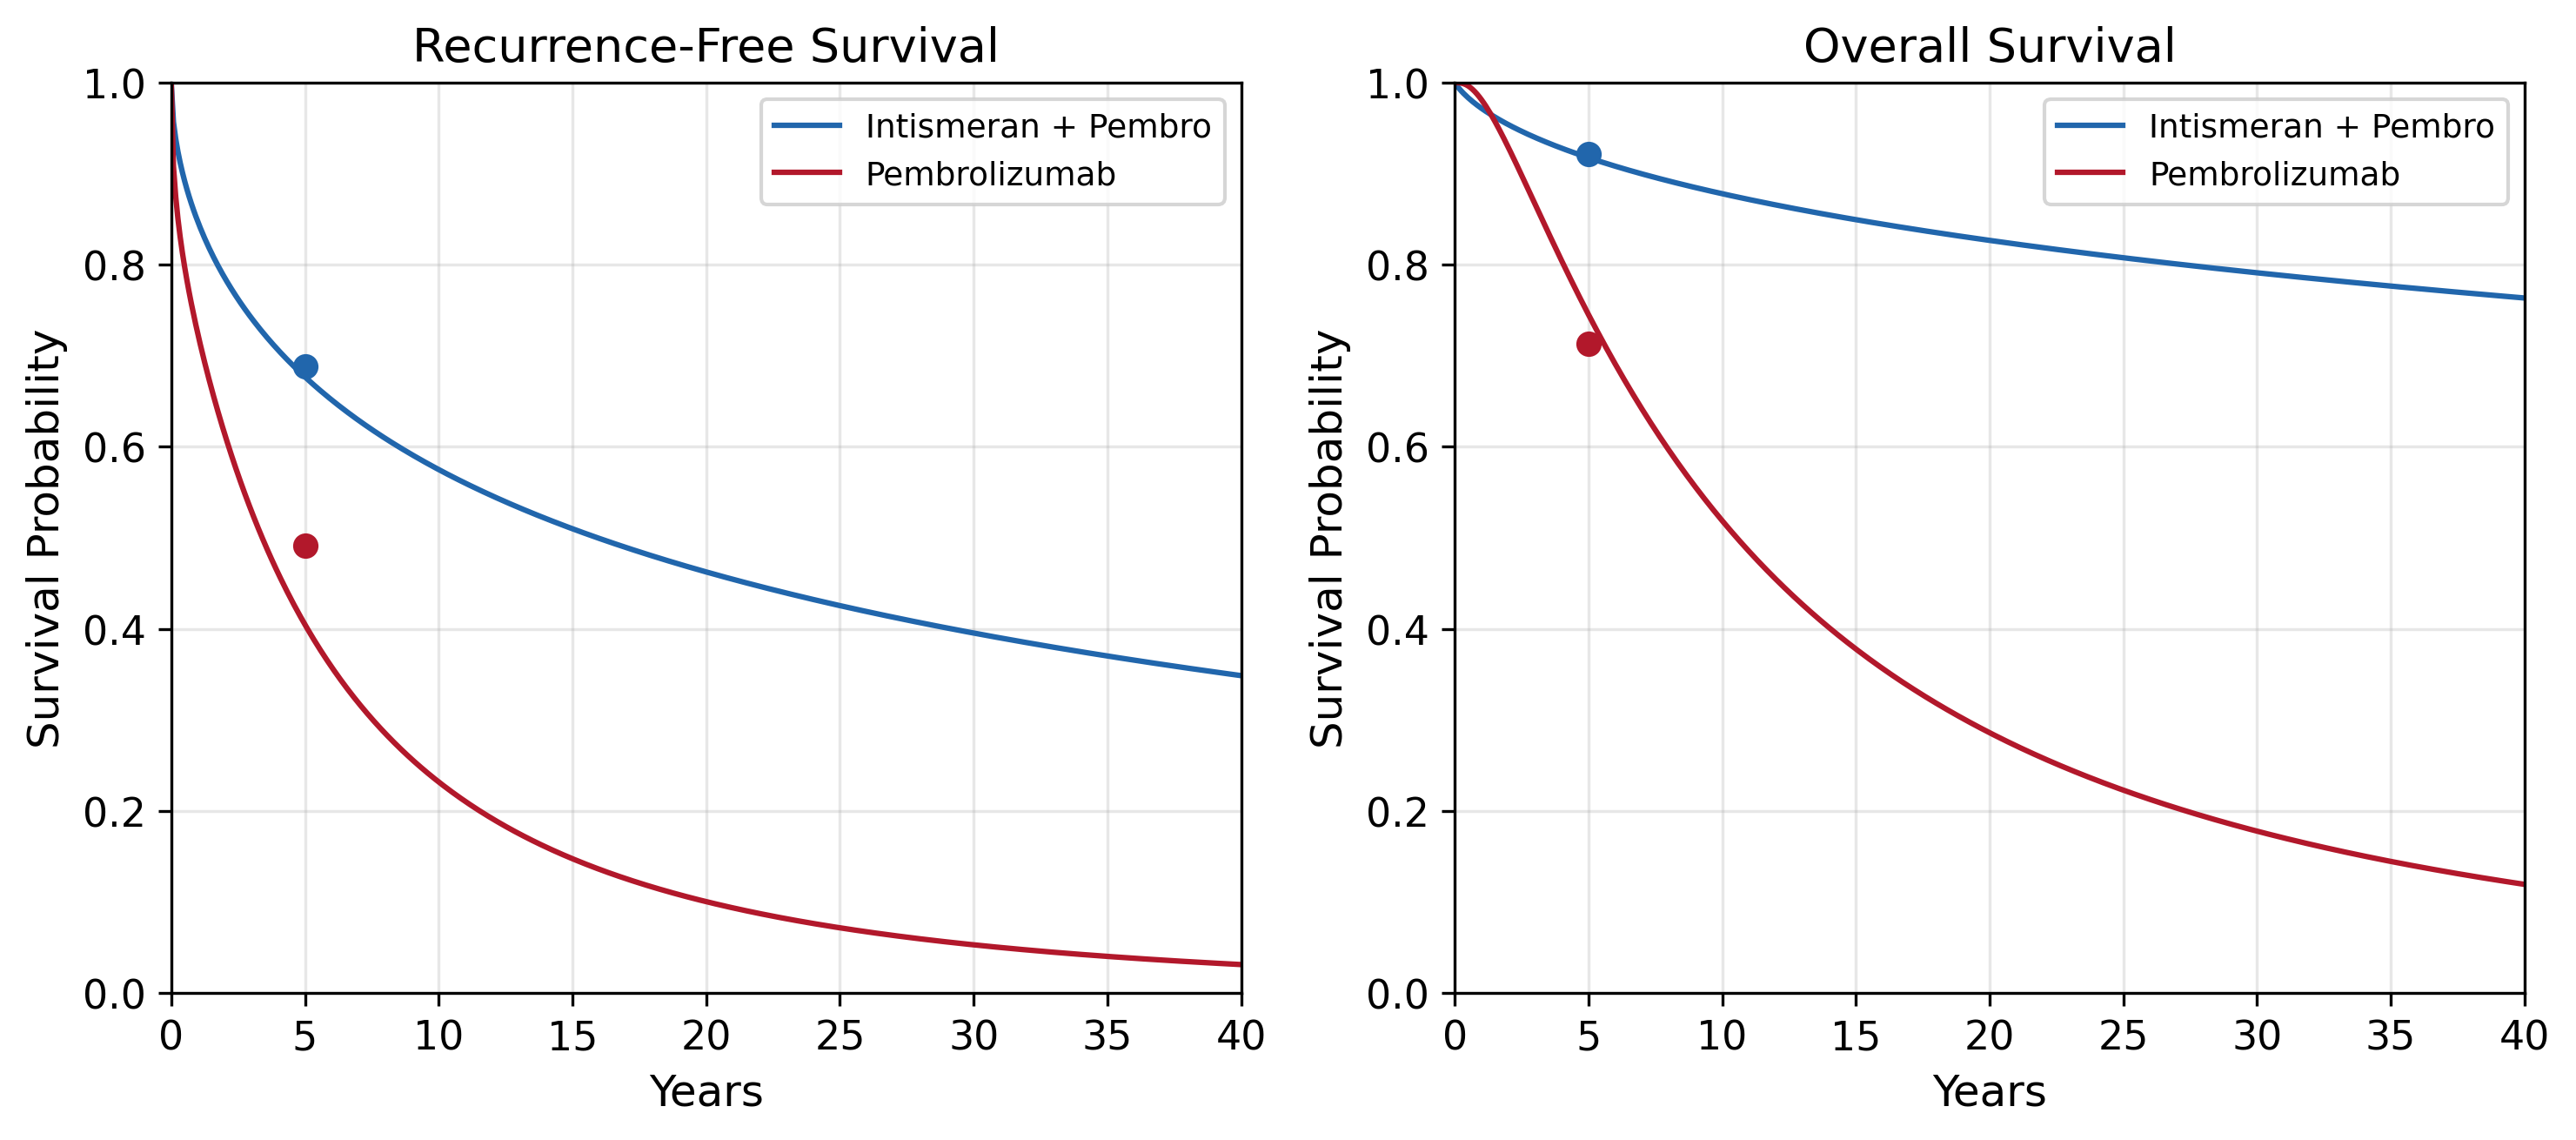
\includegraphics[width=\textwidth]{fig1_survival.png}
\caption{Partitioned survival model: RFS, DMFS, and OS curves, with data points from \mbox{KEYNOTE-942}. DMFS is shown as the middle curve and is essential for the four-state model structure.}
\label{fig:survival}
\end{figure}




\subsection{Costs}

The analysis adopted a US payer perspective. Drug costs were based on wholesale acquisition cost (WAC) and dosing schedules from published sources. Keytruda\textregistered{} (\mbox{pembrolizumab}) was assumed at 200 mg every 3 weeks for up to 18 cycles at a WAC of \$12,272 per 200 mg dose, yielding an annual cost of \$220,896 \cite{keytruda2026}. Intismeran was modeled at an assumed course acquisition price of \$200,000 based on Jefferies analyst estimates \cite{jefferies2026}.

Administration costs were included for intravenous infusions (\$500 per cycle, based on the CMS Physician Fee Schedule \cite{cms2025}). Adverse event costs were incorporated at \$15,000 incremental for the combination arm, based on published melanoma cost-effectiveness analyses \cite{bensimon2019,zhang2023}. In the \mbox{KEYNOTE-942} 5-year safety analysis, treatment-related Grade~3--5 adverse events occurred in 25.0\% of combination-arm patients and 14.0\% of \mbox{pembrolizumab}-arm patients (Supplementary Table A4, \cite{khattak2026}). Monthly disease management costs were \$3,000 for the locoregional recurrence state (salvage surgery and adjuvant therapy amortized) and \$12,000 for the distant metastasis state (systemic therapy for advanced melanoma), consistent with published melanoma CEA literature \cite{bensimon2019,zhang2023}. All costs were inflated to 2026 USD using the medical care component of the Consumer Price Index \cite{bls2025}.

\begin{table}[H]
\centering
\caption{Model Input Parameters}
\label{tab:inputs}
\begin{tabular}{lcc}
\toprule
\textbf{Parameter} & \textbf{Base Case} & \textbf{Source} \\
\midrule
5-year RFS, combo   & 68.8\%            & \mbox{KEYNOTE-942} \cite{khattak2026} \\
5-year RFS, pembro  & 49.1\%            & \mbox{KEYNOTE-942} \cite{khattak2026} \\
RFS HR              & 0.51 (95\% CI 0.294--0.887) & \mbox{KEYNOTE-942} \cite{khattak2026} \\
DMFS HR             & 0.411 (95\% CI 0.200--0.843) & \mbox{KEYNOTE-942} \cite{khattak2026} \\
OS HR               & 0.471 (95\% CI 0.165--1.345) & \mbox{KEYNOTE-942} \cite{khattak2026} \\
5-year OS, combo    & 92.2\%            & \mbox{KEYNOTE-942} \cite{khattak2026} \\
5-year OS, pembro   & 71.3\%            & \mbox{KEYNOTE-942} \cite{khattak2026} \\
Keytruda annual cost & \$220,896        & WAC \cite{keytruda2026} \\
Intismeran course cost & \$200,000       & Jefferies \cite{jefferies2026} \\
\bottomrule
\end{tabular}
\end{table}


\subsection{Utilities}

Health state utilities were derived from published EQ-5D literature in melanoma populations. The base case utilities were: RF 0.83, LR 0.64, and DM 0.55 \cite{bensimon2019, johnston2021, zhang2023}. A one-time utility decrement of 0.05 was applied for adverse events in the combination arm, consistent with published melanoma CEA literature.

\subsection{Base Case Analysis}

The base case analysis was conducted over a lifetime horizon (40 years) with 3\% annual discounting for both costs and QALYs, following the recommendations of the Second Panel on Cost-Effectiveness in Health and Medicine \cite{sanders2016}. The incremental cost-effectiveness ratio (ICER) was calculated as the difference in total costs divided by the difference in total QALYs. Cost-effectiveness was evaluated at willingness-to-pay thresholds of \$50,000, \$100,000, and \$150,000/QALY \cite{neumann2014}.

\subsection{Sensitivity Analysis}

Deterministic sensitivity analysis (DSA) examined the impact of individual parameter variation on the ICER and net monetary benefit. Parameters were varied one at a time across plausible ranges: survival model parameters, health-state utilities, costs, and the discount rate (Table~\ref{tab:inputs}).

Probabilistic sensitivity analysis (PSA) was conducted with 6,000 Monte Carlo iterations to propagate joint parameter uncertainty \cite{briggs2006}. Survival parameters $(\mu, \sigma)$ for all six underlying curves (OS, $r_{\text{DM}}$, $r_{\text{LR}}$, each for the combination and \mbox{pembrolizumab} arms) were jointly sampled from bivariate normal distributions with covariance matrices derived from the nonlinear least-squares Jacobian (Supplementary Table~S12). This approach approximates parameter uncertainty from the landmark-based nonlinear fits and therefore does not fully reproduce the sampling uncertainty of the original censored trial data; the 95\% confidence intervals from PSA should be interpreted as reflecting curve-fit uncertainty rather than the full statistical uncertainty that would be obtained from individual patient-level data. Cross-arm covariance could not be estimated from the published aggregate Kaplan--Meier data; arm-specific survival parameters were therefore sampled independently. No specific cross-arm correlation was imposed because such a parameter could not be identified without patient-level data. Scale parameters ($\sigma$) were sampled on the log-scale and lower-truncated at 0.05 to ensure positivity; any draw producing $\sigma \leq 0$ was automatically rejected and redrawn. Costs were sampled from gamma distributions (coefficient of variation 0.2), and utilities from beta distributions (standard error 0.03). The intismeran acquisition price was held fixed at \$200,000 in all iterations, as the price had not yet been announced at the time of analysis; its impact was instead explored through deterministic threshold pricing (Section~3.6) and scenario analysis (Table~4). Structural constraints (RFS $\leq$ DMFS $\leq$ OS, monotonicity, survival within [0,1]) were verified in every iteration; no iterations were excluded on the basis of the ICER value, and all 6,000 draws satisfied the structural validity criteria (0 rejections). Results are reported as mean incremental net monetary benefit (NMB) and cost-effectiveness probability at each willingness-to-pay threshold, following recommended practice \cite{stinnett1998, fenwick2004}. Convergence was verified by checking that cumulative means stabilised by approximately 500 iterations (Supplementary Figure~S6).

\section{Results}

\subsection{Base-Case Clinical and Economic Outcomes}

In the base case with general population mortality constraint, intismeran plus \mbox{pembrolizumab} generated an additional 4.78 discounted life-years (15.06 vs 10.28) and 4.02 additional QALYs (11.35 vs 7.33 QALYs) compared with \mbox{pembrolizumab} alone, at an incremental lifetime cost of \$161,916 (\$874,026 vs \$712,110). This yielded an ICER of \$40,274/QALY gained (Table~\ref{tab:base}). At a willingness-to-pay threshold of \$100,000/QALY, the incremental net monetary benefit was \$240,123; at \$150,000/QALY, it was \$441,143 (Table~\ref{tab:base}).



NMB, net monetary benefit (=$\lambda \times$ QALYs $-$ cost, where $\lambda$ is the willingness-to-pay threshold) \cite{stinnett1998}.


\subsection{Cost and QALY Decomposition}

The \$200,000 acquisition cost of intismeran contributed substantially to the incremental cost. Under the corrected general-population mortality inputs, the combination arm had \$16,114 higher locoregional-recurrence management costs (\$85,455 vs \$69,341) but \$70,199 lower distant-metastasis management costs (\$354,189 vs \$424,388) than the \mbox{pembrolizumab}-alone arm, because \mbox{pembrolizumab}-alone patients spend more time in the DM state over the lifetime (1.62 vs 1.35 discounted DM QALYs). The incremental QALY gain of 4.02 was driven primarily by additional time spent in the recurrence-free state (4.01 RF QALYs gained), with a modest additional 0.29 LR QALYs, partly offset by a 0.27-QALY reduction in the DM state.

\begin{table}[H]
\centering
\caption{Base-Case Results and Decomposition}
\label{tab:base}
\begin{tabular}{lccc}
\toprule
\textbf{Component} & \textbf{Combo} & \textbf{Pembro} & \textbf{Incremental} \\
\midrule
\multicolumn{4}{c}{\textit{Cost decomposition}} \\
Intismeran   & \$200,000   & \$0        & \$200,000 \\
Pembrolizumab & \$217,888  & \$217,888  & \$0 \\
Sequencing   & \$1,000     & \$0        & \$1,000 \\
Administration/AE & \$15,493 & \$493    & \$15,000 \\
LR management & \$85,455  & \$69,341   & \$16,114 \\
DM management & \$354,189  & \$424,388  & $-$70,199 \\
\midrule
Total cost    & \$874,026 & \$712,110  & \$161,916 \\
\midrule
\multicolumn{4}{c}{\textit{QALY decomposition}} \\
RF state      & 8.49       & 4.48       & 4.01 \\
LR state      & 1.52       & 1.23       & 0.29 \\
DM state      & 1.35       & 1.62       & $-$0.27 \\
\midrule
Total QALYs   & 11.35      & 7.33       & 4.02 \\
\bottomrule
\end{tabular}
\end{table}

\subsection{External and Structural Validation}

Survival extrapolation was validated along two dimensions: internal structural consistency of the PSM framework, and external calibration of the \mbox{pembrolizumab} arm against published adjuvant melanoma evidence.

\paragraph{Structural consistency.} Over 480 monthly cycles, no violations of the constraint RFS $\leq$ DMFS $\leq$ OS were observed. All health-state probabilities remained non-negative, and the sum of state probabilities was within $10^{-12}$ of unity at every cycle. The general population mortality hazard floor, applied from 60 months onward, ensures that the model's long-term survival does not exceed age- and sex-matched US life-table survival at any time point. At 30 years, the model projects combo OS of 22.2\% and pembro OS of 10.5\%, both below the general-population survival of 23.1\% at 30 years for the modeled cohort (baseline age 61, pooled 64\% male), consistent with the hazard-floor property that a cohort with a history of excess mortality remains below the general-population curve.

\paragraph{External plausibility assessment.} The \mbox{pembrolizumab}-alone arm predictions were compared against published long-term landmark values from two external adjuvant melanoma trials \cite{eggermont2025,ascierto2025}. At 5 years, the model predicted RFS of 40.5\%, DMFS of 53.8\%, and OS of 74.5\% for the \mbox{pembrolizumab} arm. The predicted 5-year OS (74.5\%) was consistent with the observed \mbox{KEYNOTE-942} value (71.3\%) and with the 5-year OS of 76\% in CheckMate 238 \cite{ascierto2023}. At 7 years, the model predicted RFS of 31.9\% and DMFS of 44.9\%, below the KEYNOTE-054 7-year values (RFS 50\%, DMFS 54\%) \cite{eggermont2025}; the absolute differences were $-$18.1 and $-$9.1 percentage points, respectively. The 5-year RFS of 40.5\% was $-$10.5 percentage points relative to the CheckMate 238 5-year RFS of 51\%. This divergence is consistent with the higher-risk population enrolled in \mbox{KEYNOTE-942} (stage IIIB--IV including resected stage IV vs IIIA--C in KEYNOTE-054), though other factors such as differences in clinical practice and trial design may also contribute. Only published landmark values were used; no external trial extrapolations were employed. Because the \mbox{pembrolizumab} arm serves as the comparator for the incremental analysis, its under-prediction of RFS may, if anything, overstate the incremental QALY gain attributable to intismeran; however, the direction of any bias is not straightforward, as the model's predicted OS for the \mbox{pembrolizumab} arm was close to observed (74.5\% vs 71.3\% at 5 years). No external long-term data exist for the combination arm (first-in-class therapy). Instead of relying on this comparison to calibrate the base case, scenario analyses that directly bound the treatment effect --- treatment-effect waning and no-direct-OS-benefit (Section~3.5) --- were used to bound the range of plausible ICER estimates.



\subsection{Probabilistic and Deterministic Uncertainty}

Probabilistic sensitivity analysis. Probabilistic sensitivity analysis across 6,000 structurally valid iterations (0 rejections) quantified joint parameter uncertainty. The probability of cost-effectiveness increased with the willingness-to-pay threshold, from 63.8\% at \$50,000/QALY to 95.3\% at \$100,000/QALY and 98.7\% at \$150,000/QALY. Figure~\ref{fig:ceac} presents the cost-effectiveness acceptability curve across the full range of willingness-to-pay thresholds. All 6,000 iterations produced positive incremental QALYs, and 16.7\% were cost-saving. Because cost-saving draws have an undefined ICER, incremental net monetary benefit and probability of cost-effectiveness are the preferred summary statistics (Table~\ref{tab:psa}) \cite{stinnett1998}.

\begin{table}[H]
\centering
\caption{Probabilistic Sensitivity Analysis}
\label{tab:psa}
\begin{tabular}{lrrr}
\toprule
\textbf{Metric} & \textbf{Mean} & \textbf{Median} & \textbf{95\% CI} \\
\midrule
Incremental cost  & \$127,711 & \$165,479 & $-$\$668,394 to \$520,672 \\
Incremental QALYs & 4.32      & 4.15      & 2.53--7.04 \\
NMB @ \$100,000/QALY & \$304,291 & --- & --- \\
NMB @ \$150,000/QALY & \$520,293 & --- & --- \\
\bottomrule
\end{tabular}
\end{table}

\begin{figure}[H]
\centering
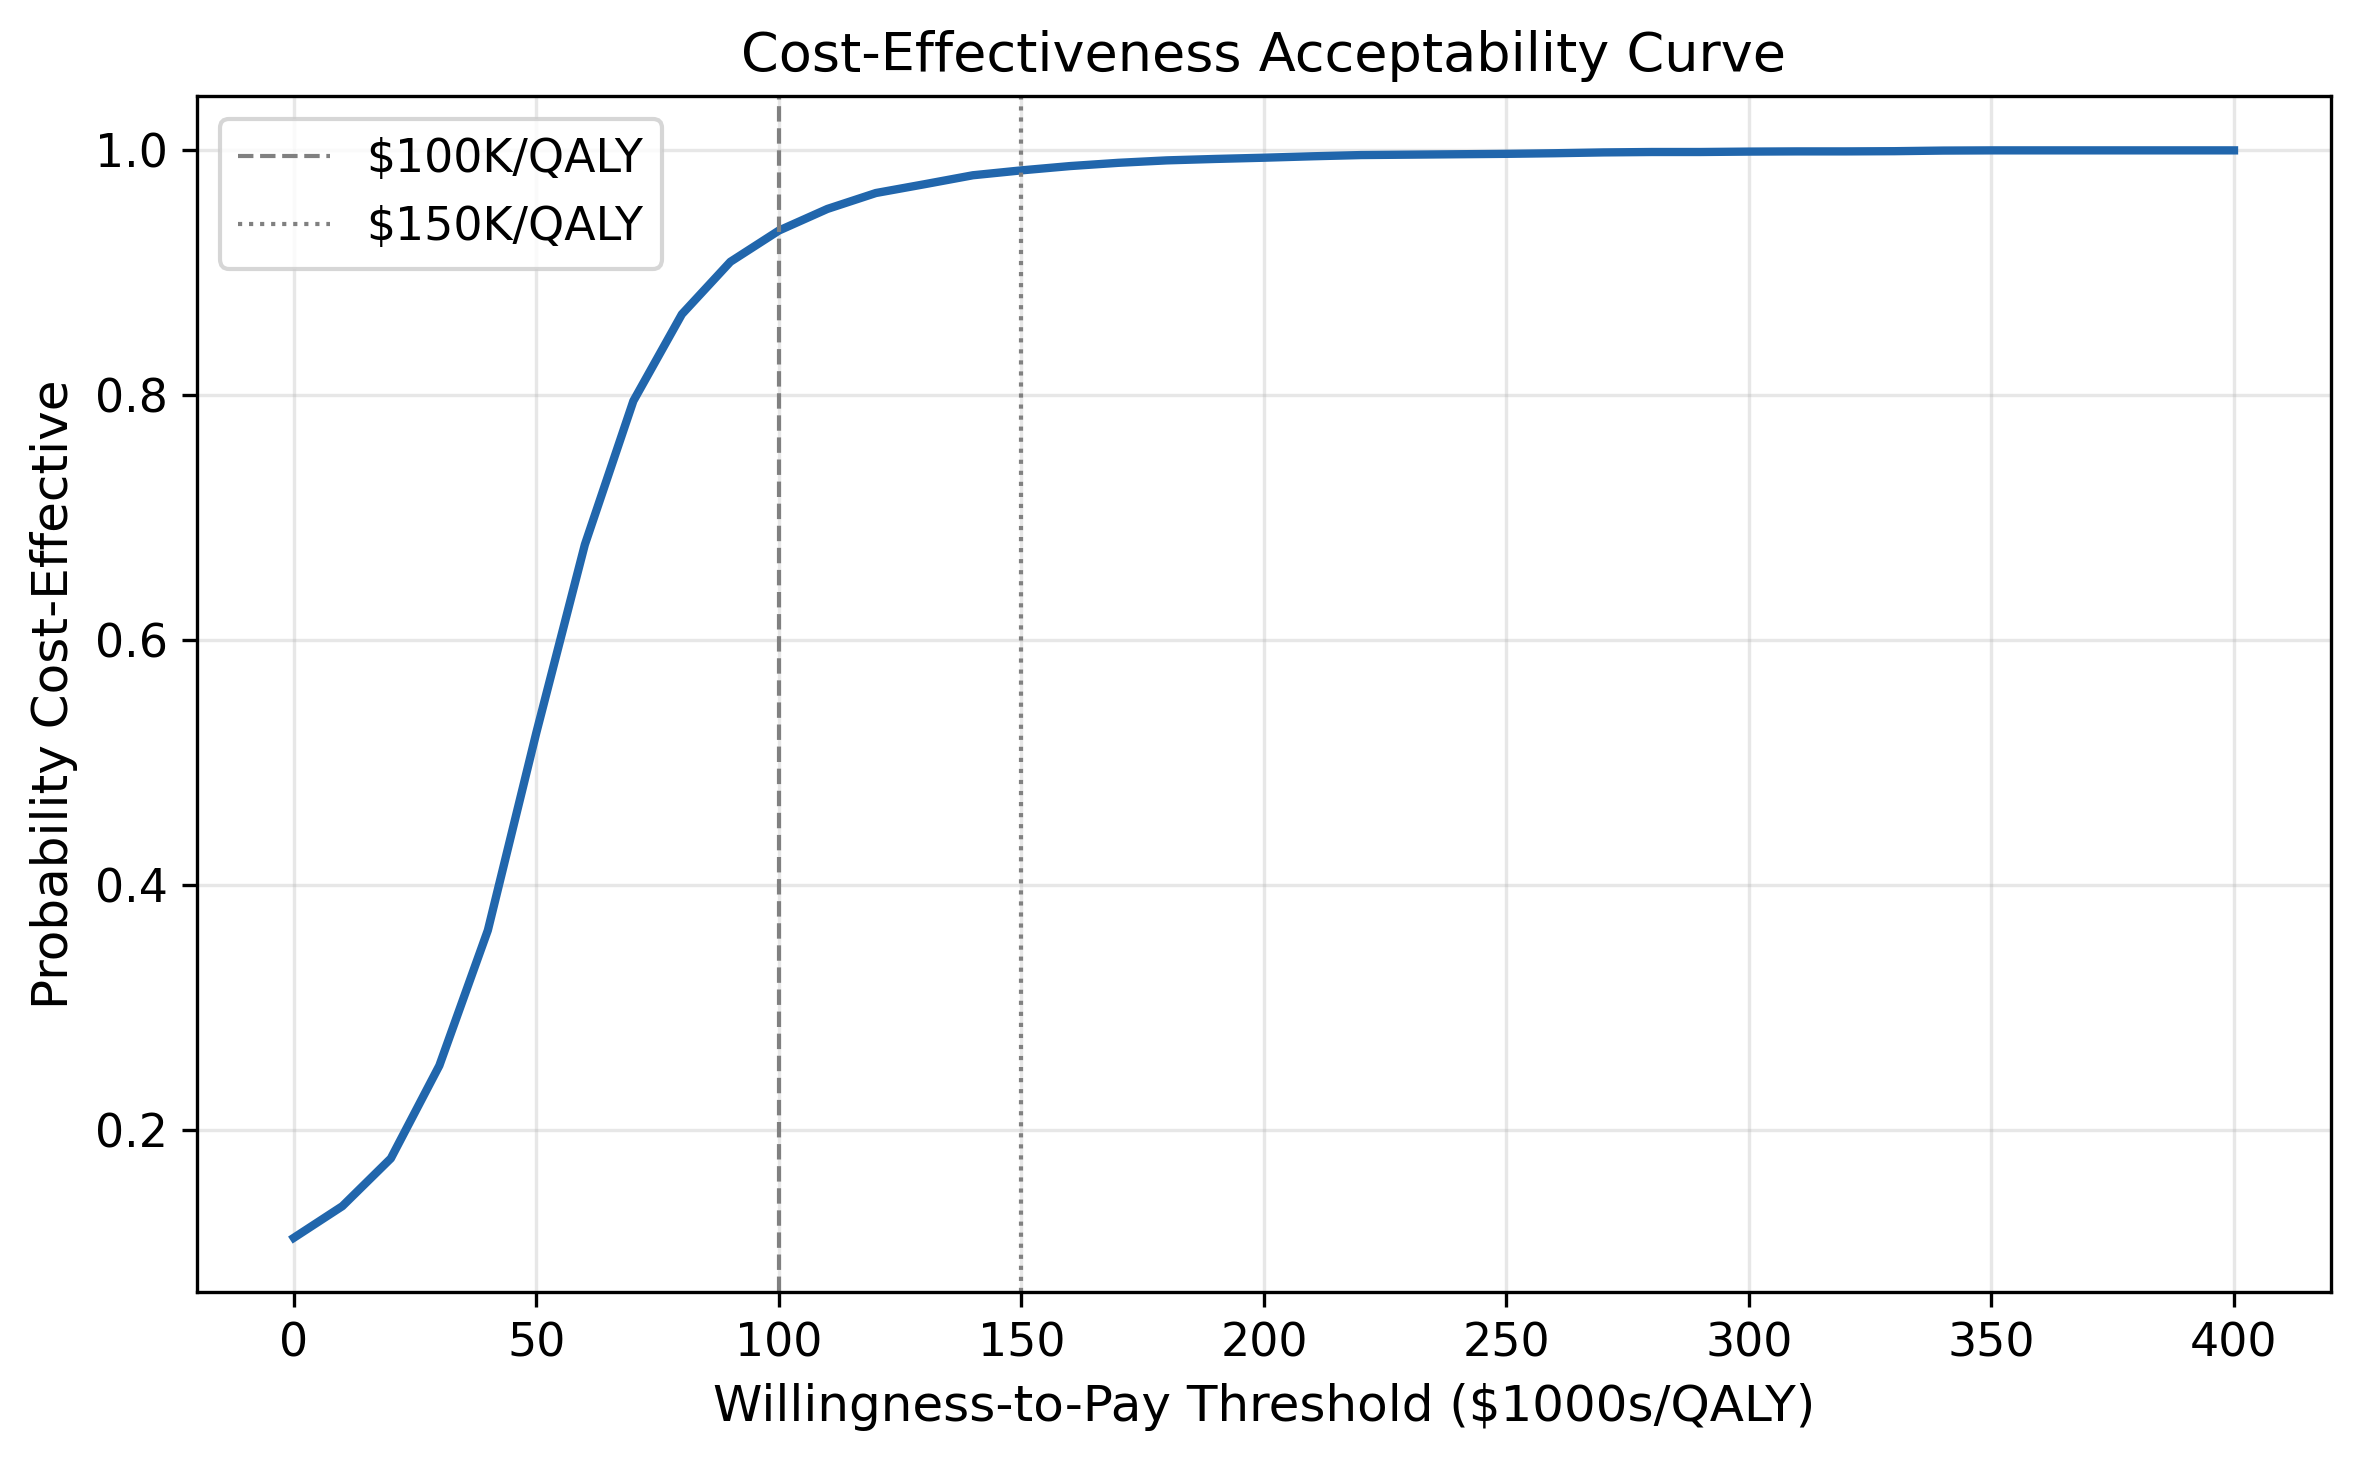
\includegraphics[width=\textwidth]{fig2_ceac.png}
\caption{Cost-effectiveness acceptability curve.}
\label{fig:ceac}
\end{figure}



Deterministic sensitivity analysis. One-way sensitivity analysis identified the parameters with the greatest influence on the base-case ICER (Supplementary Table~S11). As shown in Figure~\ref{fig:tornado}, the largest NMB changes arose from the combination-arm OS parameter (ICER \$19,875--\$40,684/QALY across its $-40\%$ to $+40\%$ range), the \mbox{pembrolizumab}-arm OS parameter (\$57,434/QALY to dominant across its $-20\%$ to $+20\%$ range), and the discount rate (\$33,120--\$48,284/QALY across 0\%--5\%). The intismeran acquisition-price range produced ICERs of \$30,324--\$50,223/QALY. Across the tested ranges, the maximum finite ICER was \$57,434/QALY; under the high \mbox{pembrolizumab} OS parameter value, the combination became dominant.

\begin{figure}[H]
\centering
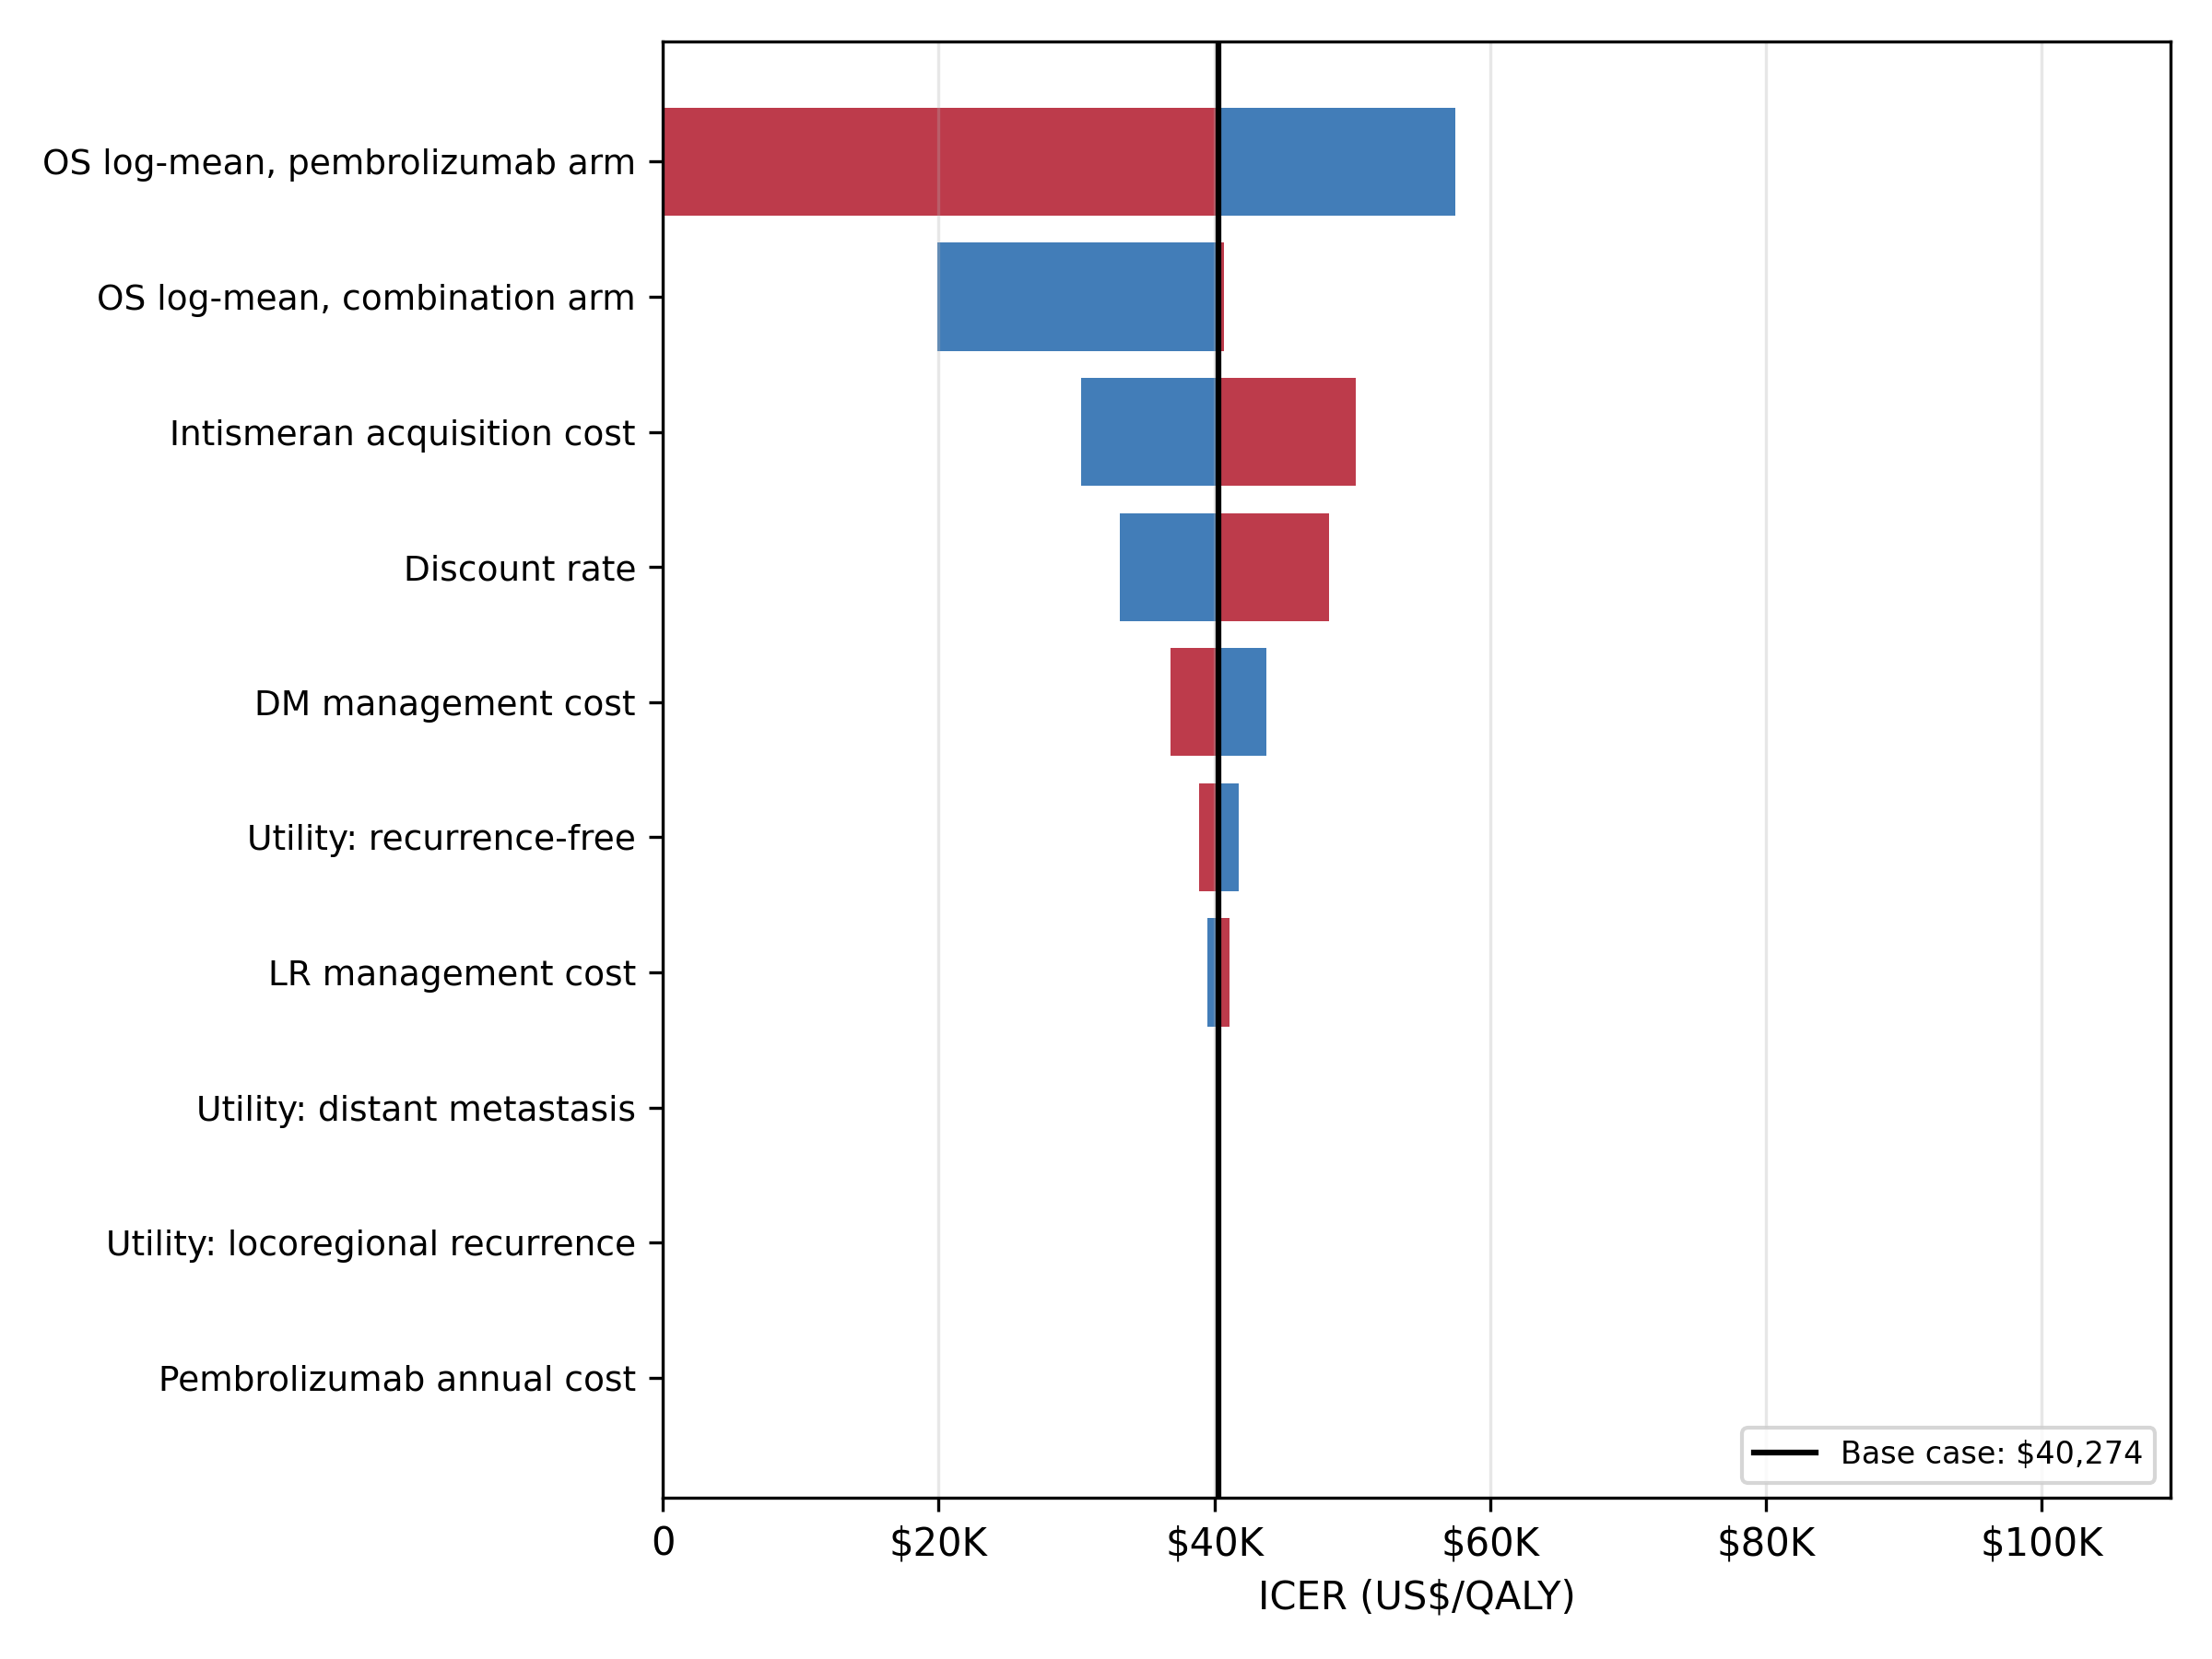
\includegraphics[width=\textwidth]{fig3_tornado.png}
\caption{Tornado diagram of one-way sensitivity analysis.}
\label{fig:tornado}
\end{figure}


\subsection{Structural Scenario Analyses}

Scenario analysis results are summarized in Table~\ref{tab:scenarios}.

\begin{table}[H]
\centering
\caption{Scenario and Deterministic Threshold Acquisition Price Analyses}
\label{tab:scenarios}
\small
\setlength{\tabcolsep}{4pt}
\begin{tabularx}{\textwidth}{@{}>{\raggedright\arraybackslash}Xrrrr@{}}
\toprule
\textbf{Scenario} & \textbf{$\Delta$ Cost} & \textbf{$\Delta$ QALY} & \textbf{ICER} & \textbf{NMB @ \$150K} \\
\midrule
Base case (GP-constrained) & \$161,916 & 4.02 & \$40,274 & \$441,143 \\
\addlinespace
\multicolumn{5}{c}{\textit{Pricing}} \\
Price: \$100K/course & \$61,916 & 4.02 & \$15,400 & \$541,143 \\
Price: \$300K/course & \$261,916 & 4.02 & \$65,147 & \$341,143 \\
Price: \$500K/course & \$461,916 & 4.02 & \$114,893 & \$141,143 \\
\addlinespace
\multicolumn{5}{c}{\textit{Alternative assumptions}} \\
Weibull OS & \$307,578 & 5.60 & \$54,925 & \$532,420 \\
Discount rate: 0\% & \$210,821 & 6.37 & \$33,120 & \$743,990 \\
Discount rate: 5\% & \$147,137 & 3.05 & \$48,284 & \$309,960 \\
Time horizon: 10 years & \$96,400 & 1.30 & \$74,305 & \$33,335 \\
Time horizon: 20 years & \$123,974 & 3.08 & \$40,293 & \$337,545 \\
\addlinespace
\multicolumn{5}{c}{\textit{Treatment-effect persistence}} \\
OS-survival convergence (5\textendash20y) & \$41,571 & 1.93 & \$21,514 & \$248,268 \\
Hazard convergence (5\textendash10y) & \$227,542 & 2.17 & \$104,852 & \$97,975 \\
No direct OS benefit & \textendash\$14,330 & 0.50 & Dominant & \$89,330 \\
\bottomrule
\end{tabularx}
\end{table}
\subsection{Deterministic Threshold Acquisition Price}

At the assumed base-case acquisition price of \$200,000 per course, the ICER was \$40,274/QALY. Figure~\ref{fig:price_icer} shows the relationship between intismeran acquisition price and the ICER, with the curve crossing the \$100,000/QALY and \$150,000/QALY thresholds at approximately \$440,000 and \$641,000 per course, respectively.

\begin{figure}[H]
\centering
\includegraphics[width=\textwidth]{fig4_price_icer.png}
\caption{Price--ICER curve and deterministic threshold pricing. Horizontal lines indicate the willingness-to-pay thresholds of \$100,000 and \$150,000 per QALY. Vertical reference lines indicate the base-case price (\$200,000) and the deterministic threshold prices at \$100,000/QALY and \$150,000/QALY.}
\label{fig:price_icer}
\end{figure}


\section{Discussion}

\subsection{Principal Findings}

This early economic evaluation suggests that intismeran plus \mbox{pembrolizumab} was projected to be cost-effective under the base-case assumptions for adjuvant treatment of resected stage IIIB--IV melanoma at conventional US willingness-to-pay thresholds. The base case ICER of \$40,274/QALY, the 4.02 QALY gain, and the 95.3\% probability of cost-effectiveness at \$100,000/QALY (98.7\% at \$150,000/QALY) all support this conclusion. Notably, under the modeled recurrence effects and health-state cost and utility assumptions, the combination remained dominant (lower cost and higher QALY) in the scenario where intismeran provided no direct OS benefit beyond its effect on recurrence. This scenario indicates that favorable economics can be supported by recurrence prevention alone within the model, rather than establishing that the conclusion is independent of OS assumptions.

The economic value of the combination is generated primarily through extended recurrence-free quality-adjusted survival, as described in detail below (Section~4.2). The ICER is notably lower than the \$75,206 from the prior exploratory analysis \cite{mclean2024} (Section~4.5), reflecting the combined effect of mature clinical data and a structurally constrained modelling framework.

\subsection{Economic Drivers and Cost Consequences}

The incremental \$161,916 lifetime cost of intismeran plus \mbox{pembrolizumab} is partly offset by lower distant-metastasis management costs, because the combination arm prevents recurrence and metastatic disease despite its \$200,000 acquisition cost. The QALY decomposition (Table~\ref{tab:base}) shows that the 4.02 incremental QALYs are driven primarily by additional time in the recurrence-free health state (4.01 RF QALYs), with a modest additional 0.29 LR QALYs and 0.27 fewer DM-state QALYs. Thus, the favorable ICER reflects a large gain in recurrence-free quality-adjusted survival together with lower lifetime distant-metastasis management costs, which partially offset the acquisition cost.

\subsection{Pricing and Reimbursement Implications}

The base case assumes an intismeran acquisition price of \$200,000 per course, based on Jefferies analyst estimates. At this price, the ICER of \$40,274/QALY is well below conventional US thresholds. The deterministic threshold price analysis (Section~3.6) shows that the ICER remains below \$100,000/QALY at intismeran prices up to approximately \$440,000 per course and below \$150,000/QALY up to approximately \$641,000 per course, providing a deterministic cost-effectiveness benchmark under the base-case assumptions.

While individualized production requirements --- including tumor sequencing, mRNA synthesis, lipid nanoparticle formulation, and quality assurance for each batch --- may contribute to acquisition-price pressure, production cost and commercial price are distinct quantities. The \$200,000 estimate reflects the expected market price at launch, not the manufacturer's cost of goods sold. Several factors may reduce future production costs: sequencing costs continue to decline \cite{schwarze2020}, mRNA platform manufacturing is becoming increasingly standardized, and automation of the synthesis and formulation pipeline could reduce per-batch costs. However, whether these technical efficiencies will translate into lower acquisition prices for payers is uncertain, as pricing decisions are influenced by clinical value, competitive dynamics, and reimbursement negotiations, not solely by production economics.

Cost-effectiveness should not be conflated with affordability. The deterministic threshold price of approximately \$440,000 per course at \$100,000/QALY implies that the combination could be considered cost-effective at more than twice the current estimated price, but the incremental cost of adding \$200,000 in drug costs to an already expensive \mbox{pembrolizumab} regimen would be substantial in a population of eligible patients. Formal budget-impact analysis is needed alongside cost-effectiveness evidence for reimbursement decision-making. Given the uncertainty surrounding long-term effectiveness and the eventual commercial price of intismeran, managed-entry or outcomes-based reimbursement arrangements may be relevant at launch. Their design, however, would require mature Phase 3 efficacy data, an announced acquisition price, and clearly defined measurable outcomes.

\subsection{Long-Term Survival and Structural Uncertainty}

Long-term survival extrapolation is the dominant source of structural uncertainty in this analysis. The mature 5-year RFS and DMFS data from \mbox{KEYNOTE-942} provide a robust foundation for the recurrence and metastasis components of the model, but OS remains exploratory (HR 0.471; 95\% CI 0.165--1.345; 7 events per arm) and must be extrapolated to a lifetime horizon. The model's 40-year combination-arm survival of 2.0\% (Table~S6) is a structural consequence of the fitted parametric model combined with the general-population mortality hazard floor and should not be interpreted as a clinical prediction of survival to age 101; no melanoma trial has followed patients beyond approximately 8 years, and this long-term trajectory should be interpreted as a modeling assumption.

The necessity of the general population mortality hazard floor is best illustrated by comparing the constrained and unconstrained models. Without the GP mortality floor, the log-normal survival fit for the combination arm predicts a 30-year OS of 79.1\%, far exceeding the age- and sex-matched general population survival of 23.1\% at 30 years for the modeled cohort. This is implausible: a cohort of patients with resected stage IIIB--IV melanoma cannot have a lower mortality rate than the general population. Applying the GP mortality hazard floor from 60 months onward --- a standard practice recommended by NICE DSU TSD 14 \cite{latimer2011} and used in published melanoma CEAs \cite{zhang2023} --- reduces the 30-year combination OS to 22.2\%, a clinically plausible trajectory. The hazard floor reduces the ICER from \$51,753 (unconstrained) to \$40,274 (GP-constrained); the direction of this change is non-intuitive (the constraint reduces the ICER) because the unconstrained model predicts implausibly high survival for both arms, with a larger absolute gain for the combination arm, and the hazard floor compresses that difference while preserving the within-trial benefit.

The OS uncertainty is further underscored by the treatment-effect waning scenarios (see Supplementary Section~9.3 for technical implementation definitions). In the OS-survival convergence scenario (5$\to$20y), the ICER falls to \$21,514/QALY because the incremental OS benefit is progressively eliminated, while the \$200,000 intismeran acquisition cost is preserved -- the incremental cost therefore drops from \$161,916 to \$41,571 faster than QALYs, producing a lower ICER. The hazard-convergence scenario (5$\to$10y) yields the highest ICER of \$104,852/QALY. These two scenarios bracket the range of plausible ICER estimates under alternative treatment-persistence assumptions.

Finally, the choice of parametric distribution, while important, is secondary to the structural scenarios. The log-normal distribution was selected by AIC for the combination OS curve and was applied uniformly across all components for parsimony. However, AIC measures fit within the observed 5-year follow-up; it does not establish long-term clinical validity. The Weibull alternative, which produced an ICER of \$54,925/QALY, also satisfied the structural constraints and is a plausible alternative. The most informative bounds on the ICER come not from alternative parametric forms but from the treatment-effect waning and no-direct-OS-benefit scenarios, which directly address the question: what if the treatment effect does not persist? The best AIC-ranked mixed-family combination (OS: log-normal/Weibull, r$_{\text{DM}}$: log-normal/log-logistic, r$_{\text{LR}}$: log-logistic/Weibull) produced an ICER of \$61,102, consistent with the Weibull scenario and within the range of structural uncertainty, further supporting the robustness of the base-case conclusion.

\subsection{Comparison with Previous Economic Evaluations}

Direct comparison of ICERs across adjuvant melanoma cost-effectiveness studies is not straightforward, because the incremental decision differs. Bensimon et al.\ \cite{bensimon2019} and Zhang et al.\ \cite{zhang2023} evaluated \mbox{pembrolizumab} versus observation, estimating the value of adding immunotherapy to surveillance. The present analysis evaluates intismeran plus \mbox{pembrolizumab} versus \mbox{pembrolizumab} alone, estimating the incremental value of adding an individualized neoantigen vaccine to an already active immunotherapy regimen. The relevant policy question is therefore not whether the combination is cost-effective in absolute terms, but whether the combination of two active agents can provide sufficient additional clinical value to justify the acquisition cost of the second agent after accounting for the lower lifetime distant-metastasis management costs in the combination arm.

The ICER of \$40,274/QALY is within the range of published estimates for the initial \mbox{pembrolizumab} decision (\$38,050--\$78,400/QALY), but this comparability is coincidental rather than meaningful. The absolute QALY gain from adding intismeran to \mbox{pembrolizumab} (4.02 QALYs) is larger than the gain from adding \mbox{pembrolizumab} to observation (1.2--2.1 QALYs in Bensimon and Zhang), because the comparator arm (\mbox{pembrolizumab} alone) has already been optimized through immunotherapy. The incremental cost is also larger (\$161,916 vs approximately \$100,000--\$150,000). The ratio happens to fall within a similar range because both numerator and denominator increase proportionally, not because the value proposition is comparable.

The comparison with the 2024 exploratory analysis \cite{mclean2024} is more informative but requires careful interpretation. That analysis, conducted before the Phase 3 \mbox{INTerpath-001} readout, assumed V940 priced at parity with \mbox{pembrolizumab}, applied \mbox{KEYNOTE-942} hazard ratios to external \mbox{pembrolizumab} survival curves from KEYNOTE-054, and used a single parametric distribution per endpoint. The present analysis differs on all four dimensions: post-Phase III evidence context, direct fitting to \mbox{KEYNOTE-942} 5-year data, a \$200,000 price assumption, and a ratio-constrained structural framework with a general population mortality floor. The lower ICER (\$40,274 vs \$75,206) is the net result of these four differences, not a univariate effect of any single factor, and should not be interpreted as evidence that intismeran is simply more effective than previously estimated.

\subsection{Clinical and External Validity}

The \mbox{pembrolizumab}-alone arm predictions were compared against published long-term adjuvant melanoma data to assess the plausibility of the extrapolated survival trajectories, rather than to require an exact match. The \mbox{KEYNOTE-942} trial enrolled a higher-risk population (stage IIIB--IV, including resected stage IV) than KEYNOTE-054 (stage IIIA--C) and CheckMate 238 (stage IIIB--IV, but with different entry criteria). The model's lower 7-year RFS for the \mbox{pembrolizumab} arm (31.9\% vs 50\% in KEYNOTE-054) is directionally consistent with the higher-risk population enrolled in \mbox{KEYNOTE-942}, though the magnitude of the difference ($-$18.1 percentage points) suggests that population risk alone may not fully explain the divergence; differences in clinical practice, trial design, and measurement protocols may also contribute. The model closely reproduced the 5-year OS of the \mbox{pembrolizumab} arm, while its RFS and DMFS projections were evaluated against available trial landmarks and external adjuvant melanoma evidence.

No external long-term data exist for the combination arm (first-in-class therapy). The positive Phase 3 \mbox{INTerpath-001} readout provides directional confirmation of the clinical benefit of intismeran plus \mbox{pembrolizumab}, but the numerical hazard ratios have not yet been disclosed, and the extent to which Phase 3 results will align with the Phase 2b \mbox{KEYNOTE-942} estimates used in this model remains to be determined. Two structural scenarios address the uncertainty in the combination arm: (i) the treatment-effect waning scenarios --- OS-survival convergence at 5$\to$20y (ICER \$21,514/QALY, most favourable) and hazard-convergence at 5$\to$10y (ICER \$104,852/QALY, least favourable); and (ii) the no-direct-OS-benefit scenario, an OS-neutral structural scenario in which intismeran plus \mbox{pembrolizumab} remained dominant (lower cost and higher QALY) compared with \mbox{pembrolizumab} alone, under the modeled recurrence effects and health-state cost and utility assumptions, indicating that recurrence prevention alone can support favorable economics within the model but does not establish independence from the model assumptions.

\subsection{Limitations}

This analysis has several limitations that should be considered when interpreting the results. First, this early economic evaluation derives efficacy inputs from Phase 2b \mbox{KEYNOTE-942} (n=157). Subsequent positive Phase 3 \mbox{INTerpath-001} readout (n=1,137) confirmed RFS and DMFS benefit; model inputs will be updated as Phase 3 numerical data become available. Second, overall survival data from \mbox{KEYNOTE-942} remain exploratory, with an HR of 0.471 (95\% CI 0.165--1.345) and only 7 events per arm at the 5-year analysis, and the 5-year OS estimate of 92.2\% versus 71.3\% should be interpreted with caution. Third, survival curves were reconstructed from published Kaplan--Meier figures using digitized coordinates rather than being estimated from individual patient-level data, which introduces measurement error in the parametric fits. Fourth, survival extrapolation beyond the observed 5-year follow-up, while structurally constrained and anchored to a general population mortality floor, remains sensitive to the choice of parametric distribution and the assumption that the treatment effect persists indefinitely. In particular, the projected 40-year combination-arm OS of 2.0\% is a model extrapolation, not a clinically observed estimate, and the base-case ICER should be read alongside the 20-year horizon result (\$40,293/QALY) as a more conservative benchmark. Time horizon sensitivity analysis showed that the ICER remained below conventional US willingness-to-pay thresholds at 20, 30, and 40 years (\$40,293, \$39,914, and \$40,274/QALY, respectively), although the point estimate increased with longer extrapolation, indicating that the 40-year extrapolation window did not materially drive the base-case results. Fifth, the intismeran acquisition price of \$200,000 per course is based on analyst estimates, and the actual market price may differ. Sixth, wholesale acquisition cost (WAC) was used for \mbox{pembrolizumab}, which may not reflect confidential net prices after rebates and discounts. Because \mbox{pembrolizumab} costs were applied symmetrically to both arms, plausible reductions in its net price would have limited impact on the incremental cost comparison. Seventh, health-state utilities and disease management costs for the LR and DM states were drawn from published melanoma CEA literature rather than prospectively collected from \mbox{KEYNOTE-942}, and may not fully capture the experience of the modeled population. Eighth, indirect costs, productivity losses, and informal caregiver burden were not included, which may underestimate the societal value of preventing recurrence and distant metastasis in a working-age population. Ninth, the \mbox{KEYNOTE-942} trial enrolled a mixed-stage population (IIIB--IV), and baseline recurrence risk varies substantially by disease stage. The Phase 2b sample size precluded formal subgroup cost-effectiveness analysis by stage, PD-L1 status, or other risk factors. If the treatment effect differs by baseline risk, the average ICER may not reflect the value of intismeran in specific subgroups, and reimbursement decisions would ideally consider stage-specific estimates. The Phase 3 \mbox{INTerpath-001} trial (N=1,137, stage IIB--IV) will provide sufficient statistical power for subgroup analyses, and the present findings should be updated when those data become available. Tenth, no formal budget-impact analysis was conducted; the cost-effectiveness findings should be complemented by an affordability assessment when pricing and population-level data become available. Any future population-level budget exposure calculations should be explicitly labeled as illustrative and not interpreted as formal budget-impact analyses, which require detailed market uptake, incident cohort, and annual expenditure modeling. Finally, this analysis is specific to the resected stage IIIB--IV melanoma population of \mbox{KEYNOTE-942} and may not be generalizable to other melanoma stages or tumor types, although the Phase 3 \mbox{INTerpath-001} trial enrolled a broader stage IIB--IV population.

\subsection{Conclusion}

Intismeran plus \mbox{pembrolizumab} provides clinical benefit in adjuvant melanoma and was projected to be cost-effective at the estimated acquisition cost of \$200,000 per course under the base-case assumptions. The deterministic threshold price analysis shows that the ICER remains below \$100,000/QALY at intismeran prices up to approximately \$440,000 per course, providing a deterministic cost-effectiveness benchmark under the base-case assumptions. The large QALY gain from extended recurrence-free survival represents clinical benefit, while lower distant-metastasis management costs partially offset the acquisition cost. As more mature data become available from the Phase 3 \mbox{INTerpath-001} trial, these findings should be updated.

\section*{Declarations}

\textbf{Conflict of interest:} The author declares no competing interests relevant to this study.

\textbf{Reporting:} This study adheres to the Consolidated Health Economic Evaluation Reporting Standards 2022 (CHEERS 2022) \cite{husereau2022} (Supplementary Checklist).

\textbf{Data availability:} All data used in this analysis are derived from published sources cited in the references. The model code is available at \url{https://github.com/yichao2022/cea-intismeran}.

\textbf{Code availability:} The partitioned survival model was implemented in Python and is available at \url{https://github.com/yichao2022/cea-intismeran}.

\textbf{Author contributions:} Yichao Jin conceived and designed the study, developed the model, conducted the analysis, and wrote the manuscript.

% --- References ---
\newpage
\bibliography{refs}

\end{document}